\pagestyle{empty}

% =========================================================================
% KHỐI 1: KẾT THÚC VÍ DỤ TRƯỚC (DÓNG HÀNG HÌNH 4 VÀ ĐOẠN LỜI GIẢI)
% =========================================================================
\noindent
\begin{minipage}[t]{0.23\textwidth}
  \vspace{0pt}
  \centering
  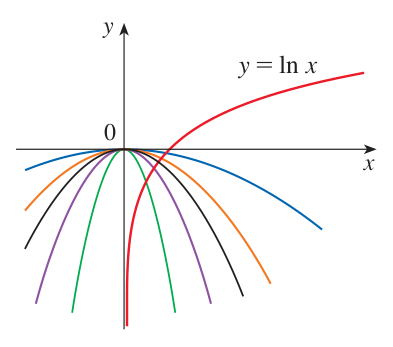
\includegraphics[width=\linewidth]{images/p0310_fig1.png}
  
  \vspace{3pt}
  {\raggedright\textsf{\textbf{\footnotesize HÌNH 4}}\par}
\end{minipage}%
\hfill
\begin{minipage}[t]{0.73\textwidth}
  \vspace{0pt}
  Giải hệ phương trình $\ln a = ca^2$ và $1/a = 2ca$, ta được
  \begin{equation*}
    \ln a = ca^2 = c\left(\frac{1}{2c}\right) = \frac{1}{2}
  \end{equation*}
  Do đó $a = e^{1/2}$ và
  \begin{equation*}
    c = \frac{\ln a}{a^2} = \frac{\ln e^{1/2}}{e} = \frac{1}{2e}
  \end{equation*}
  Với các giá trị âm của $c$, ta có tình huống được minh họa trong Hình~4: tất cả các parabol $y = cx^2$ với giá trị $c$ âm đều cắt $y = \ln x$ tại đúng một điểm. Và cũng đừng quên trường hợp $c = 0$: đường cong $y = 0x^2 = 0$ chính là trục hoành, cắt $y = \ln x$ tại đúng một điểm.

  Tóm lại, các giá trị cần tìm của $c$ là $c = 1/(2e)$ và $c \leqslant 0$. \hfill {\color{stewartcyan}$\blacksquare$}
\end{minipage}

\vspace{14pt}

% =========================================================================
% KHỐI 2: MỤC BÀI TOÁN (PROBLEMS) VÀ HÌNH MINH HỌA BÀI 8
% =========================================================================
\noindent
\begin{minipage}[t]{0.23\textwidth}
  \vspace{0pt}
  % Thanh tiêu đề Bài toán
  \begin{tcolorbox}[
    colback=stewartlightpurple, 
    colframe=stewartlightpurple, 
    arc=1.5mm, 
    left=6pt, 
    right=6pt, 
    top=3.5pt, 
    bottom=3.5pt, 
    boxrule=0pt,
    width=\linewidth
  ]
    {\textsf{\textbf{\color{stewartpurple}\large Bài toán}}}
  \end{tcolorbox}

  \vspace{255pt}
  % Hình cho bài toán 8 (dóng chính xác ngang bài 8)
  \centering
  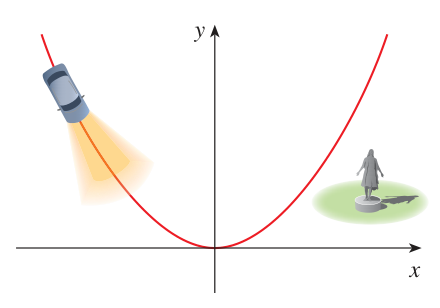
\includegraphics[width=\linewidth]{images/p0310_fig3.png}
  
  \vspace{3pt}
  {\raggedright\textsf{\textbf{\footnotesize HÌNH CHO BÀI TOÁN 8}}\par}
\end{minipage}%
\hfill
\begin{minipage}[t]{0.73\textwidth}
  \vspace{0pt}
  \setlength{\abovedisplayskip}{3.5pt}
  \setlength{\belowdisplayskip}{3.5pt}
  \begin{list}{}{%
    \setlength{\labelwidth}{15pt}%
    \setlength{\leftmargin}{15pt}%
    \setlength{\itemindent}{0pt}%
    \setlength{\itemsep}{5.5pt}%
    \setlength{\parsep}{0pt}%
    \setlength{\topsep}{0pt}%
  }
    \item[\textbf{1.}] Tìm các điểm $P$ và $Q$ trên parabol $y = 1 - x^2$ sao cho tam giác $ABC$ tạo bởi trục hoành và các tiếp tuyến tại $P$ và $Q$ là một tam giác đều (xem hình vẽ).

    \begin{center}
      \vspace{-2pt}
      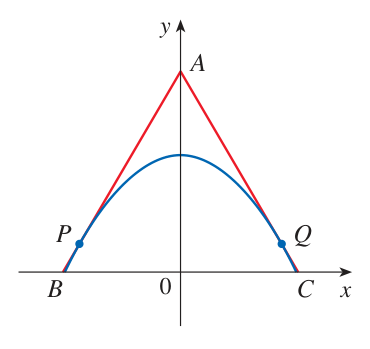
\includegraphics[width=0.40\linewidth]{images/p0310_fig2.png}
      \vspace{-2pt}
    \end{center}

    \item[{\makebox[0pt][r]{\graphingicon\hspace{3.5pt}}\textbf{2.}}] Tìm điểm mà tại đó hai đường cong $y = x^3 - 3x + 4$ và $y = 3(x^2 - x)$ tiếp xúc với nhau, nghĩa là có chung một tiếp tuyến. Minh họa bằng cách phác thảo cả hai đường cong và tiếp tuyến chung.

    \item[\textbf{3.}] Chứng minh rằng các tiếp tuyến của parabol $y = ax^2 + bx + c$ tại hai điểm bất kỳ có hoành độ $p$ và $q$ phải cắt nhau tại một điểm có hoành độ nằm chính giữa $p$ và $q$.

    \item[\textbf{4.}] Chứng minh rằng $\dfrac{d}{dx}\left(\dfrac{\sin^2 x}{1 + \cot x} + \dfrac{\cos^2 x}{1 + \tan x}\right) = -\cos 2x$.

    \item[\textbf{5.}] Nếu $f(x) = \lim\limits_{t \to x}\dfrac{\sec t - \sec x}{t - x}$, hãy tìm giá trị của $f'(\pi/4)$.

    \item[\textbf{6.}] Tìm các giá trị của các hằng số $a$ và $b$ sao cho
    \begin{equation*}
      \lim_{x \to 0} \frac{\sqrt[3]{ax + b} - 2}{x} = \frac{5}{12}
    \end{equation*}

    \item[\textbf{7.}] Chứng minh rằng $\sin^{-1}(\tanh x) = \tan^{-1}(\sinh x)$.

    \item[\textbf{8.}] Một chiếc ô tô đang di chuyển vào ban đêm dọc theo một đường cao tốc có hình dạng parabol với đỉnh tại gốc tọa độ (xem hình bên). Xe xuất phát tại điểm cách gốc tọa độ 100~m về phía tây và 100~m về phía bắc, rồi đi về hướng đông. Có một bức tượng nằm cách gốc tọa độ 100~m về phía đông và 50~m về phía bắc. Tại điểm nào trên đường cao tốc thì đèn pha của xe sẽ chiếu thẳng vào bức tượng?

    \item[\textbf{9.}] Chứng minh rằng $\dfrac{d^n}{dx^n}(\sin^4 x + \cos^4 x) = 4^{n-1}\cos(4x + n\pi/2)$.
  \end{list}
\end{minipage}

\vfill
% Số trang
\noindent
\makebox[\textwidth][r]{\textsf{\textbf{\large 275}}}

\vspace{2pt}
% Dòng bản quyền Cengage
\noindent
{\fontsize{5}{6}\selectfont\color{stewartgray}%
Copyright 2021 Cengage Learning. All Rights Reserved. May not be copied, scanned, or duplicated, in whole or in part. Due to electronic rights, some third party content may be suppressed from the eBook and/or eChapter(s). Editorial review has deemed that any suppressed content does not materially affect the overall learning experience. Cengage Learning reserves the right to remove additional content at any time if subsequent rights restrictions require it. WCN 02-200-203\par}
